\documentclass[conference]{IEEEtran}
\usepackage[utf8]{inputenc}
\usepackage[T1]{fontenc}
\usepackage[spanish,es-tabla,es-nodecimaldot]{babel}
\usepackage{graphicx,booktabs,amsmath,cite,url,array}
\usepackage[hidelinks]{hyperref}

\begin{document}

\title{Perfil socioeconómico y desempeño en Saber~11:\\ agrupación, árboles de decisión y bandits contextuales}

\author{\IEEEauthorblockN{Camilo Alejandro Lagos Malaver, [Integrante 2], [Integrante 3]}
\IEEEauthorblockA{Introducción a los Sistemas Inteligentes, 2026-2\\
Departamento de Ingeniería de Sistemas e Industrial\\
Universidad Nacional de Colombia, Bogotá\\
\{clagosm\}@unal.edu.co}}

\maketitle

\begin{abstract}
Aplicamos tres técnicas de aprendizaje maquinal a los resultados del examen Saber~11 de 2022 (calendario~A, los 530.815 estudiantes con resultados completos) para responder dos preguntas: qué tanto explican las condiciones del hogar y del colegio el desempeño, y qué área convendría reforzar según el perfil del estudiante. K-means (Weka) separa tres perfiles cuya diferencia de puntaje global llega a 29 puntos. Un árbol de decisión J48 (Weka) predice si un estudiante queda sobre la mediana con 69,2\,\% de exactitud (AUC 0,74) frente a 50,2\,\% de la línea base, y sus primeras divisiones son tener computador, la edad y la jornada. Un bandit contextual LinUCB, que elige qué área reforzar observando solo la recompensa del área elegida, reduce el arrepentimiento 12\,\% frente al azar. Las tres técnicas coinciden: el perfil pesa, pero explica solo una parte del resultado individual.
\end{abstract}

\begin{IEEEkeywords}
Saber 11, K-means, árboles de decisión, J48, bandit contextual, LinUCB, Weka.
\end{IEEEkeywords}

\section{Introducción}
El examen Saber~11 del ICFES evalúa a quienes terminan la educación media en matemáticas, lectura crítica, sociales y ciudadanas, ciencias naturales e inglés. Además del puntaje, cada registro trae un cuestionario socioeconómico y datos del colegio. Esto permite estudiar la relación entre el contexto del estudiante y su desempeño con técnicas de los tres paradigmas vistos en el curso: aprendizaje no supervisado (agrupación), supervisado (clasificación) y por refuerzo.

Planteamos tres preguntas, una por técnica: (P1) ¿qué perfiles de estudiantes existen según su hogar y su colegio, y cómo les va? (P2) ¿qué variables permiten predecir si un estudiante queda en la mitad superior? (P3) si un tutor virtual debe elegir una sola área para reforzar a cada estudiante, ¿puede aprender a elegir mejor que al azar usando solo el perfil?

\section{Datos y preprocesamiento}
Usamos el conjunto \emph{Resultados únicos Saber 11} publicado por el ICFES en datos.gov.co (identificador \texttt{kgxf-xxbe}, licencia CC BY-SA 4.0), con 7,11 millones de registros de 2010 a 2022 y 51 columnas~\cite{icfes}. Tomamos el periodo 20224 (calendario~A de 2022). La consulta devuelve 1.065.888 filas, pero cada estudiante aparece dos veces: tras eliminar duplicados quedan 532.792 registros únicos, que coinciden con el número de consecutivos distintos. Descartamos 1.977 sin los cinco puntajes, y trabajamos con \textbf{530.815 estudiantes}.

\textbf{Atributos.} Conservamos 18 atributos de contexto: género, edad al examen (calculada de la fecha de nacimiento y discretizada en $\le$16, 17, 18, 19--20 y $>$20 años), estrato, educación de la madre y del padre (agrupada en ocho niveles; ``No sabe'' como faltante), si el hogar tiene internet, computador, automóvil y lavadora, personas y cuartos del hogar, y del colegio: naturaleza (oficial o no), área (urbano o rural), jornada, bilingüe, carácter, género y departamento. Se descartaron identificadores, nombres y códigos. Los faltantes (entre 0 y 18\,\% según la columna) se dejaron como \texttt{?} para que Weka los maneje.

\textbf{Clase.} Para la clasificación definimos \emph{Alto} si el puntaje global supera la mediana (247 puntos) y \emph{Bajo} en otro caso, lo que da clases balanceadas.

\textbf{Todos los datos.} El preprocesamiento se hizo en Python con pandas y se exportó a ARFF. Las tres técnicas usan los 530.815 estudiantes, sin muestreo; Weka se ejecutó por línea de comandos con 6~GB de memoria. Una corrida preliminar con una muestra aleatoria de 150.000 dio exactitudes casi iguales (J48: 68,5\,\% frente a 69,2\,\%); la diferencia principal está en los grupos de K-means.

\section{Técnica 1: agrupación con K-means}
\subsection{Método}
Usamos \texttt{SimpleKMeans} de Weka 3.8.6~\cite{weka} con los 17 atributos de perfil (sin departamento y \emph{sin la clase}). Con atributos nominales, Weka usa la moda como centroide y cuenta coincidencias como distancia; los faltantes se reemplazan por la moda. Probamos $k=2,\dots,8$ y elegimos $k$ con el método del codo sobre la suma de errores intra-grupo (SSE). Luego usamos \emph{classes to clusters} y comparamos el puntaje de cada grupo.

\begin{figure}[t]
\centering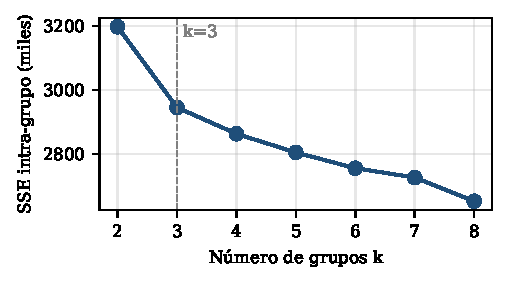
\includegraphics[width=\columnwidth]{fig/codo.pdf}
\caption{SSE intra-grupo de K-means en Weka para $k=2,\dots,8$.}
\label{fig:codo}
\end{figure}

\subsection{Resultados}
La SSE baja de 3.198.180 ($k=2$) a 2.945.619 ($k=3$) y después mejora poco (2.863.264 con $k=4$), así que elegimos $k=3$ (Fig.~\ref{fig:codo}). La Tabla~\ref{tab:grupos} y la Fig.~\ref{fig:grupos} describen los grupos:
\begin{itemize}
\item \textbf{G1, rural/estrato~1 sin conexión} (29,4\,\%): 58\,\% estrato~1, 30\,\% en colegio rural, solo 31\,\% con internet y 10\,\% con computador. Puntaje medio 231,0; 33,6\,\% quedan en Alto.
\item \textbf{G2, urbano conectado, mayoría mujeres} (34,7\,\%): 86\,\% con internet, 68\,\% con computador, 21\,\% en colegio privado, 69\,\% mujeres. Puntaje medio 256,9; 55,5\,\% en Alto.
\item \textbf{G3, urbano conectado, mayoría hombres} (36,0\,\%): 82\,\% con internet, 69\,\% con computador, 34\,\% en colegio privado, 29\,\% mujeres. Puntaje medio 259,8; 57,4\,\% en Alto.
\end{itemize}

\begin{table}[t]
\caption{Perfil de los grupos de K-means ($k=3$, 530.815 estudiantes)}
\label{tab:grupos}
\centering\small\setlength{\tabcolsep}{4pt}
\begin{tabular}{lrrr}
\toprule
 & G1 & G2 & G3 \\
\midrule
Tamaño (\%) & 29,4 & 34,7 & 36,0 \\
Puntaje global medio & 231,0 & 256,9 & 259,8 \\
\% en Alto & 33,6 & 55,5 & 57,4 \\
Matemáticas / Inglés & 46,6 / 44,3 & 51,8 / 51,8 & 52,8 / 52,5 \\
\% internet / computador & 31 / 10 & 86 / 68 & 82 / 69 \\
\% colegio privado / rural & 11 / 30 & 21 / 11 & 34 / 12 \\
\% mujeres & 68 & 69 & 29 \\
\bottomrule
\end{tabular}
\end{table}

\begin{figure}[t]
\centering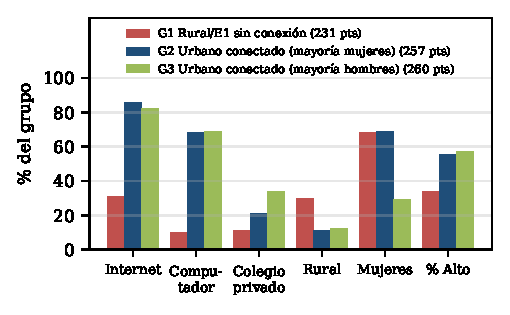
\includegraphics[width=\columnwidth]{fig/grupos.pdf}
\caption{Rasgos de cada grupo y porcentaje de estudiantes en Alto.}
\label{fig:grupos}
\end{figure}

Los grupos se formaron sin ver el puntaje y aun así ordenan el desempeño: entre G1 y G3 hay 29 puntos de diferencia. G2 y G3 tienen casi el mismo acceso a internet y computador y se separan sobre todo por género, con apenas 3 puntos de diferencia. En la muestra de 150.000 el tercer grupo era, en cambio, urbano oficial sin computador: con atributos nominales, K-means es sensible a los datos y a la inicialización, y el grupo rural sin conexión es el único estable. Como clasificador los grupos son débiles: con $k=2$, \emph{classes to clusters} asigna mal al 47,2\,\% de los estudiantes. El perfil desplaza el promedio del grupo, pero dentro de cada grupo hay mucha variación individual.

\section{Técnica 2: clasificación con árbol de decisión J48}
\subsection{Método}
J48 es la implementación de C4.5 en Weka: en cada nodo elige el atributo con mayor razón de ganancia de información y poda con un factor de confianza~\cite{quinlan}. Entrenamos dos árboles con los 18 atributos: el predeterminado (confianza 0,25 y mínimo 2 instancias por hoja, $M=2$) y uno restringido a $M=1000$ para que sea legible. Evaluamos con validación cruzada estratificada de 10 particiones contra ZeroR (predecir siempre la clase mayoritaria). Además calculamos la ganancia de información de cada atributo con \texttt{InfoGainAttributeEval}.

\subsection{Resultados}
\begin{table}[t]
\caption{Clasificación Alto/Bajo, validación cruzada de 10 particiones}
\label{tab:j48}
\centering\small
\begin{tabular}{lrrrr}
\toprule
Modelo & Exactitud & Kappa & AUC & Hojas \\
\midrule
ZeroR & 50,25\,\% & 0,000 & 0,500 & -- \\
J48, $M=2$ & 69,17\,\% & 0,383 & 0,743 & 17.091 \\
J48, $M=1000$ & 68,19\,\% & 0,364 & 0,741 & 394 \\
\bottomrule
\end{tabular}
\end{table}

Ambos árboles superan ampliamente a ZeroR (Tabla~\ref{tab:j48}). El árbol de 17.091 hojas llega a 73,4\,\% sobre los datos de entrenamiento, pero baja a 69,2\,\% en validación cruzada, señal de sobreajuste. El árbol de 394 hojas pierde solo 1,0 punto de exactitud, tiene casi el mismo AUC y se puede leer, así que lo usamos para interpretar.

La raíz es \emph{tiene computador}, seguida de la edad, la naturaleza del colegio, el área y la jornada. Algunas reglas con muchos casos:
\begin{itemize}
\item Con computador, $\le$16 años, colegio privado y jornada completa $\Rightarrow$ Alto (28.895 casos, 89\,\% de acierto).
\item Con computador, $\le$16 años, colegio oficial urbano $\Rightarrow$ Alto (83.385 casos, 67\,\%).
\item Sin computador y más de 20 años $\Rightarrow$ Bajo (11.289 casos, 89\,\%).
\item Jornadas nocturna y sabatina $\Rightarrow$ Bajo en casi todas las ramas.
\end{itemize}
La ganancia de información (Fig.~\ref{fig:ig}) coincide: los atributos más informativos son la edad (0,056 bits), la educación de la madre (0,053), la jornada (0,052) y tener computador (0,045). El estrato aparece noveno (0,021), probablemente porque su efecto ya lo capturan el computador, el internet y la educación de los padres. Que el colegio sea bilingüe o el género del estudiante casi no aportan.

\begin{figure}[t]
\centering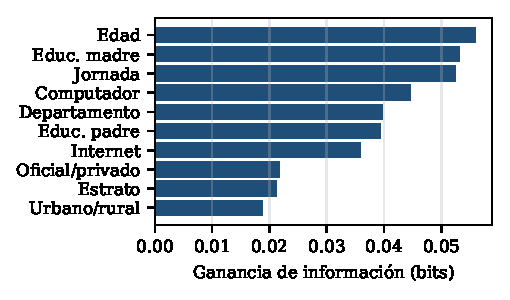
\includegraphics[width=\columnwidth]{fig/infogain.pdf}
\caption{Los 10 atributos con mayor ganancia de información respecto a la clase Alto/Bajo (Weka).}
\label{fig:ig}
\end{figure}

\section{Técnica 3: refuerzo con bandit contextual}
\subsection{Planteamiento}
Weka no incluye aprendizaje por refuerzo, así que esta parte se implementó en Python con NumPy. Modelamos un \emph{tutor virtual} que atiende estudiantes uno a uno y elige \emph{una} de cinco acciones: reforzar matemáticas, lectura, sociales, naturales o inglés. Es un \emph{bandit contextual}~\cite{li2010}: un problema de refuerzo de un solo paso donde el estado es el contexto del estudiante~\cite{sutton}.
\begin{itemize}
\item \textbf{Contexto} $x$: los 17 atributos de perfil en codificación \emph{one-hot}, más un sesgo ($d=85$).
\item \textbf{Recompensa} de la acción $a$: la brecha estandarizada del estudiante en esa área, $r_a=(\mu_a - y_a)/\sigma_a$, con $\mu_a$ y $\sigma_a$ calculadas sobre los 530.815 estudiantes. Es mayor cuanto más rezagado está el estudiante en el área elegida.
\item \textbf{Retroalimentación parcial}: el agente solo observa la recompensa del área que eligió, no la de las otras. Esto es lo que lo diferencia de la clasificación.
\end{itemize}
La acción óptima es el área más débil de cada estudiante. Medimos el \emph{arrepentimiento} acumulado, $\sum_t (\max_a r_{t,a} - r_{t,a_t})$.

\textbf{Políticas.} (i) Aleatoria; (ii) siempre matemáticas; (iii) $\varepsilon$-greedy sin contexto ($\varepsilon=0{,}05$); (iv) $\varepsilon$-greedy contextual con un modelo lineal por acción; (v) LinUCB~\cite{li2010} con $\alpha=0{,}5$, que elige $\arg\max_a \hat\theta_a^\top x + \alpha\sqrt{x^\top A_a^{-1}x}$ y actualiza $A_a^{-1}$ con la fórmula de Sherman-Morrison. Cada política recorre los 530.815 estudiantes en orden aleatorio; reportamos el promedio de tres semillas.

\subsection{Resultados}
\begin{table}[t]
\caption{Bandit contextual sobre 530.815 estudiantes (promedio de 3 semillas)}
\label{tab:bandit}
\centering\small\setlength{\tabcolsep}{4pt}
\begin{tabular}{lrrr}
\toprule
Política & Recomp. media & Arrepent. & Área óptima \\
\midrule
Aleatoria & 0,000 & 307.472 & 20,0\,\% \\
Siempre matemáticas & 0,000 & 307.645 & 20,3\,\% \\
$\varepsilon$-greedy sin contexto & 0,000 & 307.752 & 17,9\,\% \\
$\varepsilon$-greedy contextual & 0,068 & 271.624 & 24,9\,\% \\
LinUCB & \textbf{0,071} & \textbf{269.728} & \textbf{25,2\,\%} \\
Oráculo & 0,580 & 0 & 100\,\% \\
\bottomrule
\end{tabular}
\end{table}

Sin contexto no hay nada que aprender: las cinco áreas tienen recompensa media cercana a cero, y $\varepsilon$-greedy sin contexto queda igual que el azar (Tabla~\ref{tab:bandit}). Las políticas contextuales sí aprenden: LinUCB reduce el arrepentimiento 12,3\,\% frente al azar ($\varepsilon$-greedy contextual, 11,7\,\%), y la ventaja crece de forma sostenida (Fig.~\ref{fig:bandit}). LinUCB supera levemente a $\varepsilon$-greedy porque explora donde hay incertidumbre en vez de al azar.

La política aprendida es interpretable. En colegios oficiales elige inglés el 51\,\% de las veces, en zona rural el 54\,\% y en estrato~1 el 60\,\%; en colegios privados casi nunca elige inglés (0,1\,\%) y prefiere sociales (55\,\%) y matemáticas (23\,\%); en estratos 5 y 6 prioriza matemáticas y naturales. Esto coincide con el área realmente más débil en los datos: inglés es la peor área del 26,8\,\% de los estudiantes de colegio oficial y del 30,0\,\% en estrato~1, pero solo del 17,4\,\% en los privados, donde la más frecuente es matemáticas (23,7\,\%).

Aun así, la distancia al oráculo es grande (25,2\,\% frente a 100\,\% de aciertos): el perfil indica qué área tiende a ser débil en un grupo, pero no cuál es la más débil para cada persona. Una limitación es que el entorno es una simulación sobre datos fijos, por lo que la acción no cambia al estudiante.

\begin{figure}[t]
\centering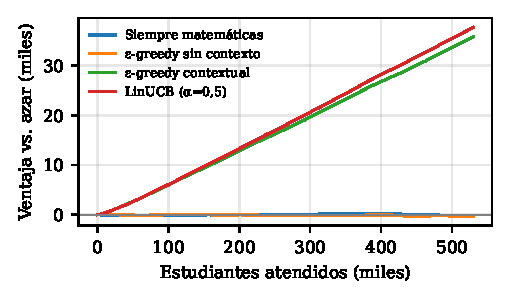
\includegraphics[width=\columnwidth]{fig/bandit.pdf}
\caption{Arrepentimiento evitado frente a la política aleatoria a medida que el agente atiende estudiantes.}
\label{fig:bandit}
\end{figure}

\section{Comparación de las técnicas}
\begin{table}[t]
\caption{Comparación de las tres técnicas}
\label{tab:comp}
\centering\footnotesize
\setlength{\tabcolsep}{3pt}\begin{tabular}{>{\raggedright\arraybackslash}p{1.4cm}>{\raggedright\arraybackslash}p{2.0cm}>{\raggedright\arraybackslash}p{2.0cm}>{\raggedright\arraybackslash}p{2.0cm}}
\toprule
 & K-means & J48 & LinUCB \\
\midrule
Paradigma & No supervisado & Supervisado & Refuerzo \\
Necesita & Solo atributos & Etiqueta Alto/Bajo & Recompensa de la acción elegida \\
Herramienta & Weka & Weka & Python \\
Pregunta & ¿Qué perfiles hay? & ¿Quién queda en Alto? & ¿Qué área reforzar? \\
Resultado & 3 grupos, 29 pts de brecha & 69,2\,\%, AUC 0,74 & $-$12\,\% arrepentimiento \\
Cómo se lee & Centroides & Reglas del árbol & Pesos por área \\
Costo (530.815) & $\approx$10 s por $k$ & 1--2 min con CV & 5,5 min (15 corridas) \\
Parámetro clave & $k$ & $M$, confianza & $\alpha$, $\varepsilon$ \\
\bottomrule
\end{tabular}
\end{table}

La Tabla~\ref{tab:comp} resume las diferencias. Las técnicas no compiten por la misma métrica, porque cada una responde una pregunta distinta con distinta información: K-means no usa el puntaje, J48 usa la etiqueta completa y el bandit solo ve la recompensa de lo que elige. Por eso, la comparación más útil es si llegan al mismo conocimiento. Y llegan:
\begin{enumerate}
\item \textbf{Las mismas variables pesan.} Computador, internet, naturaleza y área del colegio separan los grupos de K-means, encabezan el árbol J48 y cambian la política del bandit.
\item \textbf{El perfil explica una parte, no todo.} Los grupos difieren en 29 puntos pero con $k=2$ confunden al 47\,\% de los estudiantes, J48 se queda en 69,2\,\% y el bandit acierta el área óptima solo uno de cada cuatro casos.
\item \textbf{Cada técnica aporta algo propio.} K-means separa con claridad el grupo rural sin conexión y muestra que, entre los urbanos conectados, el género divide los perfiles sin cambiar mucho el puntaje; J48 muestra el peso de la edad y la jornada (la extraedad y la educación de adultos); el bandit convierte la relación en una decisión: inglés en colegios oficiales, rurales y de estrato~1; matemáticas y naturales en estratos altos.
\end{enumerate}

\section{Conclusiones}
Con los 530.815 resultados completos de Saber~11 de 2022, las tres técnicas muestran que el acceso a computador e internet, la edad, la jornada y el tipo de colegio están asociados con el desempeño. Los grupos de K-means se diferencian hasta en 29 puntos. J48 predice la mitad superior con 69,2\,\% de exactitud y deja reglas legibles. Un bandit LinUCB aprende, con retroalimentación parcial, a priorizar inglés en colegios oficiales y rurales. Ninguna técnica predice bien a cada estudiante, lo que sugiere que factores no medidos (el colegio concreto, la motivación, el docente) explican el resto. Son asociaciones, no causas, y variables como estrato o género deben usarse con cuidado para no estigmatizar grupos. Como trabajo futuro, se pueden incluir los datos del colegio específico, comparar con Random Forest y usar varios años.

\section*{Uso de inteligencia artificial}
Se usó un asistente de IA para apoyar la escritura de código y la redacción. Todos los integrantes revisaron y entienden el desarrollo, los resultados y su interpretación.

\begin{thebibliography}{9}
\bibitem{icfes} ICFES, ``Resultados únicos Saber 11,'' Datos Abiertos Colombia, conjunto \texttt{kgxf-xxbe}, 2023. [En línea]. Disponible: \url{https://www.datos.gov.co/d/kgxf-xxbe}
\bibitem{weka} E. Frank, M. A. Hall e I. H. Witten, ``The WEKA Workbench,'' apéndice en \emph{Data Mining: Practical Machine Learning Tools and Techniques}, 4.ª ed. Morgan Kaufmann, 2016.
\bibitem{quinlan} J. R. Quinlan, \emph{C4.5: Programs for Machine Learning}. San Mateo, CA: Morgan Kaufmann, 1993.
\bibitem{li2010} L. Li, W. Chu, J. Langford y R. E. Schapire, ``A contextual-bandit approach to personalized news article recommendation,'' en \emph{Proc. 19th Int. Conf. World Wide Web (WWW)}, 2010, pp. 661--670.
\bibitem{sutton} R. S. Sutton y A. G. Barto, \emph{Reinforcement Learning: An Introduction}, 2.ª ed. Cambridge, MA: MIT Press, 2018.
\end{thebibliography}

\end{document}
